

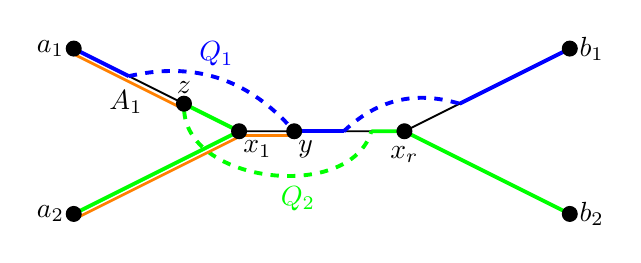
\begin{tikzpicture}[xscale=0.7, yscale=0.7]

  % vertices
  \node[draw, circle, fill=black, inner sep=1.7pt] (a1) at (-3, 1.5) {};
  \node[draw, circle, fill=black, inner sep=1.7pt] (z)  at (-1, 0.5) {};
  \node[draw, circle, fill=black, inner sep=1.7pt] (a2) at (-3, -1.5) {};
  \node[draw, circle, fill=black, inner sep=1.7pt] (x1) at (0, 0) {};
  \node[draw, circle, fill=black, inner sep=1.7pt] (y)  at (1, 0) {};
  \node[draw, circle, fill=black, inner sep=1.7pt] (xr) at (3, 0) {};
  \node[draw, circle, fill=black, inner sep=1.7pt] (b1) at (6, 1.5) {};
  \node[draw, circle, fill=black, inner sep=1.7pt] (b2) at (6, -1.5) {};
  \coordinate[inner sep=0pt] (h0) at (-2,1) {};
  \coordinate[inner sep=0pt] (h1) at (1.9,0) {};
  \coordinate[inner sep=0pt] (h2) at (2.4,0) {};  
  \coordinate[inner sep=0pt] (h3) at (4,0.5) {};  
  \coordinate[inner sep=0pt] (a1') at (-3,1.4) {};
  \coordinate[inner sep=0pt] (a2') at (-3,-1.6) {};
  \coordinate[inner sep=0pt] (z') at (-1,0.4) {};  
  \coordinate[inner sep=0pt] (x1') at (0,-0.1) {};
  \coordinate[inner sep=0pt] (x1'') at (0,-0.07) {};
  \coordinate[inner sep=0pt] (y') at (1,-0.07) {};  

  % names of vertices
%  \node[right, xshift=-6pt, yshift=7pt] at (b.north) {$b$};
  \node[left] at (a1) {$a_1$};
  \node[left] at (a2) {$a_2$};
  \node[right] at (b1) {$b_1$};
  \node[right] at (b2) {$b_2$};
  \node[above] at (z) {$z$};
  \node[below right, xshift=-2pt] at (y) {$y$};
  \node[below right, xshift=-2pt] at (x1) {$x_1$};
  \node[below, yshift=-2pt] at (xr) {$x_r$};

  % arcs
  \draw[line width=0.7pt] (a1) to node [pos=0.3, below, yshift=-2pt] {$A_1$} (x1) to (xr) to (b1);
  \draw[line width=0.7pt] (a2) to (x1);
  \draw[line width=0.7pt] (xr) to (b2);
  \draw[line width=1.4pt, blue] (a1) to (h0); 
  \draw[line width=1.4pt, blue, dashed] (h0) to [bend left=30] node[midway, above] {$Q_1$} (y); 
  \draw[line width=1.4pt, blue] (y) to (h1); 
  \draw[line width=1.4pt, blue, dashed] (h1) to [bend left=30] (h3); 
  \draw[line width=1.4pt, blue] (h3) to (b1);

  \draw[line width=1.4pt, green] (a2) to (x1) to (z);
  \draw[line width=1.4pt, green, dashed] (z) to [bend right=80] node[pos=0.6, below] {$Q_2$} (h2); 
  \draw[line width=1.4pt, green]  (h2) to (xr) to (b2);
  
  \draw[line width=1.0pt, orange] (a1') to (z');
  \draw[line width=1.0pt, orange] (a2') to (x1');
  \draw[line width=1.0pt, orange] (x1'') to (y');

  \node[draw, circle, fill=black, inner sep=1.9pt] (a1) at (-3, 1.5) {};
  \node[draw, circle, fill=black, inner sep=1.9pt] (z)  at (-1, 0.5) {};
  \node[draw, circle, fill=black, inner sep=1.9pt] (a2) at (-3, -1.5) {};
  \node[draw, circle, fill=black, inner sep=1.9pt] (x1) at (0, 0) {};
  \node[draw, circle, fill=black, inner sep=1.9pt] (y)  at (1, 0) {};
  \node[draw, circle, fill=black, inner sep=1.9pt] (xr) at (3, 0) {};
  \node[draw, circle, fill=black, inner sep=1.9pt] (b1) at (6, 1.5) {};
  \node[draw, circle, fill=black, inner sep=1.9pt] (b2) at (6, -1.5) {};

\end{tikzpicture}


















